\documentclass[10pt,twoside,a4paper]{article}

\usepackage{fancyhdr}

\usepackage{lastpage}       % ``n of m'' page numbering
\usepackage{lscape}         % Makes landscape easier

\usepackage{verbatim}       % Verbatim blocks
\usepackage{listings}       % Source code listings
\usepackage{epsfig}         % Embed encapsulated postscript
\usepackage{array}          % Array environment
\usepackage{array}          % Array environment
\usepackage{enumitem}       % Required by Tom Johnson's exam question header

\usepackage{hhline}         % Horizontal lines in tables
\usepackage{siunitx}        % Correct spacing of units
\usepackage{amsmath}        % American Mathematical Society
\usepackage{amssymb}        % Maths symbols
\usepackage{amsthm}         % Theorems

\usepackage{ifthen}         % Conditional processing in tex

\usepackage[skip=0.5cm]{parskip}

\usepackage[top=3cm,
            bottom=3cm,
            inner=2cm,
            outer=2cm]{geometry}

% If you have any additional \usepackage commands, or other
% macros or directives, put them here.  Remember not to edit
% files in the template directory because any changes will
% be overwritten when template updates are issued.
\usepackage{float,graphicx}
\usepackage{amsmath}
\usepackage{amssymb}
\usepackage{caption}
\usepackage{subfig}

\usepackage[absolute,overlay]{textpos}

\newcolumntype{C}{>$c<$}
\graphicspath{ {./images/} }

\newcommand{\notimplies}{%
  \mathrel{{\ooalign{\hidewidth$\not\phantom{=}$\hidewidth\cr$\implies$}}}}
\newcommand{\Mod}[1]{\ (\mathrm{mod}\ #1)}
\newcommand{\Z}{\mathbb{Z}}
\newcommand{\R}{\mathbb{R}}
\newcommand{\Q}{\mathbb{Q}}
\newcommand{\N}{\mathbb{N}}


\title{Delay-Tolerant Link-State Routing}
\author{Ben Andrew, ba405\\Magdalene College}
\date{\today}


\begin{document}
\maketitle


\section{Declaration of Originality}

\section{Proforma}

\section{Table of Contents}

\section{Introduction}

\section{Preparation}

\section{Implementation}

\subsection{Repository Overview}

\begin{verbatim}
dtlsr                        Root
|- configs                   CORE config files
|- include                   Include directory
|  |- algorithm
|  |- network
|  "- process
|- src                       Source directory
|  |- algorithm
|  |- network
|  "- process
|- tests                     Unit tests directory
|  |- algorithm
|  |- network
|  "- process
|- tools                     Custom development tools
"- core-py                   Custom CORE scripts
\end{verbatim}

\texttt{algorithm} contains pure algorithms and data structures, for example graph, graph searching, and heap implementations.

\texttt{network} contains functionality for socket manipulation, and sending data over the network.

\texttt{process} contains funtionality for interacting with both CORE and the Unix OS, for example retreiving node information, logging, and manipulating the Unix routing table.

The project was implemented almost entirely in C, with CORE-specific scripts in Python. I used the CMake build system and Check unit testing framework.


\subsection{CORE Background}

The Common Open Research Emulator (CORE) is a network emulator that models nodes as lightweight Unix virtual machines, complete with filesystems and network interfaces.

\begin{minipage}{1\textwidth} \centering
	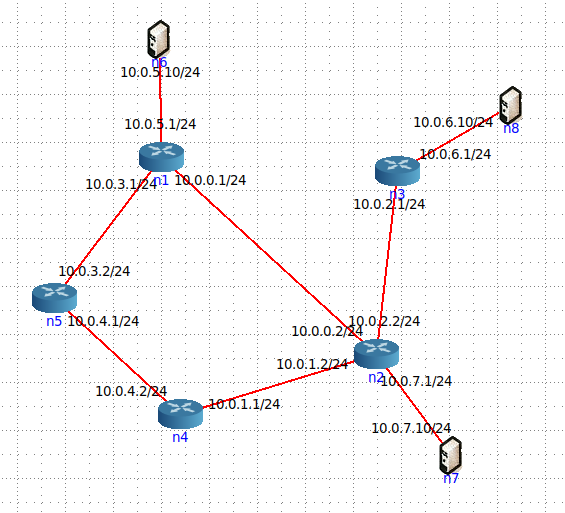
\includegraphics[width=0.6\textwidth]{6-core}
	\captionof{figure}{Example emulated network in the CORE GUI, showing routers and hosts.}
\end{minipage}

Programs can be written for these nodes and run as Unix processes via a Python API. These processes are then able to send and receive data through the emulated network via standard Unix socket programming. The emulated routers contain default routing protocol implementations, such as OSPFv2 and v3 from the Quagga protocol suite, which can be disabled and replaced by custom implementations. As well as this, standard network testing tools like \texttt{ping} can be run on emulated endpoint hosts, making testing and evaluation of the network surprisingly simple.

Link properties can be programmatically customised through the Python API, with properties including bandwidth, delay, loss, and jitter. This will aid greatly in evaluation, for example simulating network partitions.

One limitation is that CORE operates in real-time using the OS's clock, and thus the performance of the simulated network is somewhat dependent on the performance of the machine it's being run on. I will therefore be taking great care to create a reliable and statistically sound testing environment, for example setting processor priority, not running other programs, and taking baseline measurements to compare against.

\subsection{Link-State Routing Design}

The link-state routing protocol that I implemented is split into two programs, \texttt{heartbeat} and \texttt{dtlsr}. Routers run both programs, and hosts run only \texttt{heartbeat}.

\texttt{heartbeat} sends periodic heartbeat messages to all neighbouring nodes, notifying them that the connecting link is still up. The message is received by \texttt{dtlsr}. Hosts run \texttt{heartbeat} to notify their gateway router of their existence, so that the router can advertise the corresponding route.

\texttt{dtlsr} implements the bulk of the protocol. It maintains the link-state graph representation of the network, manipulates the node's routing table, and sends link-state announcements (LSAs) in response to detected changes in the network.

These changes are detected in one of three ways:
\begin{enumerate}
	\item
	A heartbeat message is received from a neighbour with a DOWN link. We set the link to be UP.
	
	\item
	A heartbeat is not received in time from a neighbour with an UP link. We set the link to be DOWN.
	
	\item
	An LSA is received from a neighbour. We merge our current graph with that of our neighbour to get the most recent information.
\end{enumerate}

Both programs lend themselves to an event-driven design, and so I used file descriptors multiplexed with the \texttt{select} Unix call to detect and respond to events. Timer file descriptors trigger when they expire and receiving socket file descriptors trigger when data arrives.

Heartbeats and LSAs are recieved on sockets with distinct ports, allowing them to be differentiated easily. While CORE supports IPv6 routing, I restricted myself to IPv4 to reduce unnecessary implementation complexity.

A heartbeat message is a UDP packet with only header, no payload. An LSA is a UDP packet whose payload is the sending node's graph representation of the network, simply copied into the payload using \texttt{memcpy}. The graph representation uses statically sized arrays rather than dynamically sized `\texttt{malloc}ed' ones, to make allocation and indexing simpler. While it would be more space-efficient to pack the graph into a more compressed structure for sending over the link, the network topologies that I use in the evaluation are not large enough for this to be an issue. It would be a simple fix if this became an issue.

\subsubsection{Local and Global Link-State}

We have two levels of representation for our network representation: a minimal global representation of the entire network and a detailed representation of the immediate neighbourhood of the local node.

For each node in the global graph, we store for each link information like the source IP, neighbour destination IP, the status of the link, the derived metric associated with the link, and a timestamp specifying how old our knowledge of that link is, for merging purposes.

The local graph consists solely of our node along with more in-depth information about links connecting us to our immediate neighbours. Along with all of the information contained in a global node, we also have for each link a timer for timing out heartbeats and the interface which that link goes out on. We take the locally-derived information and feed it into the global graph, which then gets shared with the rest of the network via LSAs.

\subsubsection{Route Generation}

Routes are derived from the link-state graph, where we compute the shortest path from ourselves to every other node in the graph using Dijkstra's algorithm. The metric for a path is given as the number of hops in the path, which I chose over a more standard OSPF-style metric depending on bandwidth as I am more concerned with delay than throughput. Notably, if a link is though to be DOWN, we disallow the pathfinding to go through that link.

After pathfinding we have for each destination address a `next-hop' address. We first generalise each specific destination address to its 24 bit subnet, zeroing out the last 8 bits. Many of these routes can then be merged together, for example if two destinations are part of a single subnet and have the same next-hop. This route aggregation reduces the size of the routing table.

We keep track of which routes we have previously added to the routing table, and mark off those that we have regenerated from the updated graph. If we have previously added routes that are not marked off, then we know that route no longer exists and we can remove it from the routing table. This may happen if a link goes down or a better alternative route appears.

With invalid routes removed, we can then add all of our new routes to the routing table. Manipulation of the Unix routing table is done through the \texttt{ioctl}, a system call for interacting with OS devices through a file descriptor interface. We pass a flag corresponding to route addition or deletion, along with a `\texttt{route}' struct containing the route details.

\subsection{Delay-Tolerant Modifications}

For the delay-tolerant version, \texttt{dtlsr} can be recompiled with the \texttt{-DDTLSR} flag active, keeping \texttt{heartbeat} identical. The modifications made are enabled/disabled simply by \texttt{\#ifdef DTLSR} preprocessor switches. Our delay-tolerant version maintains many of the same implementation design decisions as above with a few additions.

Firstly, in the pathfinding algorithm we allow routes through DOWN links so that when we update the routing table packets will be sent along the path up to the DOWN link, and buffered there until the link comes back up. The metric is modified to be, instead of hop count, an exponential time-average of the uptime history of all links along the path, so that nodes along unreliable paths will have a much higher cost. These uptime histories are maintained locally for neighbour links only; when we advertise our link state using LSAs we share only the derived metric. The metric for a path is still the summation of costs of each link along the path, which is a natural way to combine delay-dependent metrics.

An interesting edge case is when a link goes down connecting a host with its gateway router. As the host runs \texttt{heartbeat} the router will be aware that the link is down and will buffer any traffic coming in along the advertised route with the host as the destination. However any traffic the host wants to send outwards will not be buffered by itself as it is not running any `delay-tolerant' routing software; the host will have to deal with retransmissions as it will not buffer any data locally. We could theoretically develop a minimal version of the protocol that runs on hosts and only does buffering to solve this issue.

\subsubsection{Packet Buffering}

When a link is DOWN, in our delay-tolerant context we may still advertise routes going through it as if it was open, and so we may have traffic routed through us expecting to move through the link. Thus we must buffer this traffic locally until either the link comes back up or a better alternative route appears, at which point we send it on.


\subsection{Implementation Practicalities}

Some parts of the implementation were hard-coded or have inefficient solutions to aid in creating a functional piece of software that could be evaluated more quickly. These are sections that have no impact on the evaluation of the protocol as a solution to the routing problem, or are even completely unrelated to routing in general.

As an example I ran into the issue of `neighbour discovery', where nodes generally use ARP to discover the existence of neighbouring nodes on their interfaces. The ARP table in CORE proved unreliable, and as this is a link-layer problem unrelated to routing I simply hardcoded all immediate neighbours in configuration files. Implementing actual neighbour discovery would provide no practical benefits to the evaluation, and could even negatively impact it if my implementation was unreliable or had varying performance.


\section{Evaluation}

Evaluation done using CORE. Measuring end-to-end packet delay under varying network conditions. UDP and TCP.

To measure UDP performance I used \texttt{ping}, which while using ICMP emulates the behaviour of UDP well at higher throughputs, similarly having no flow and congestion control mechanisms.

We first take baseline performance measurements, of the routing convergence time for LSR and DTLSR. Both use the same routing system so should have similar results.

Measuring delay with \texttt{ping}, we use a variety of network topologies to demonstrate different properties of the routing algorithms.

Firstly we have a topology with a single central connecting link, that we flap to create a network partition. In this example we flap link \texttt{n1-n2}. Every link has \SI{1}{\ms} of delay.

\begin{minipage}{1\textwidth} \centering
	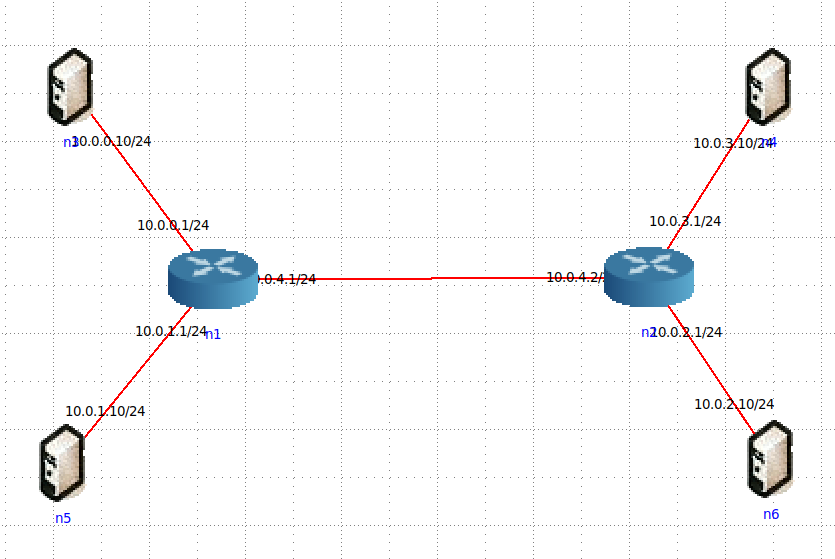
\includegraphics[width=0.7\textwidth]{partition}
	\captionof{figure}{`Partition' network topology.}
\end{minipage}

\begin{figure}
\begin{tabular}{c}
  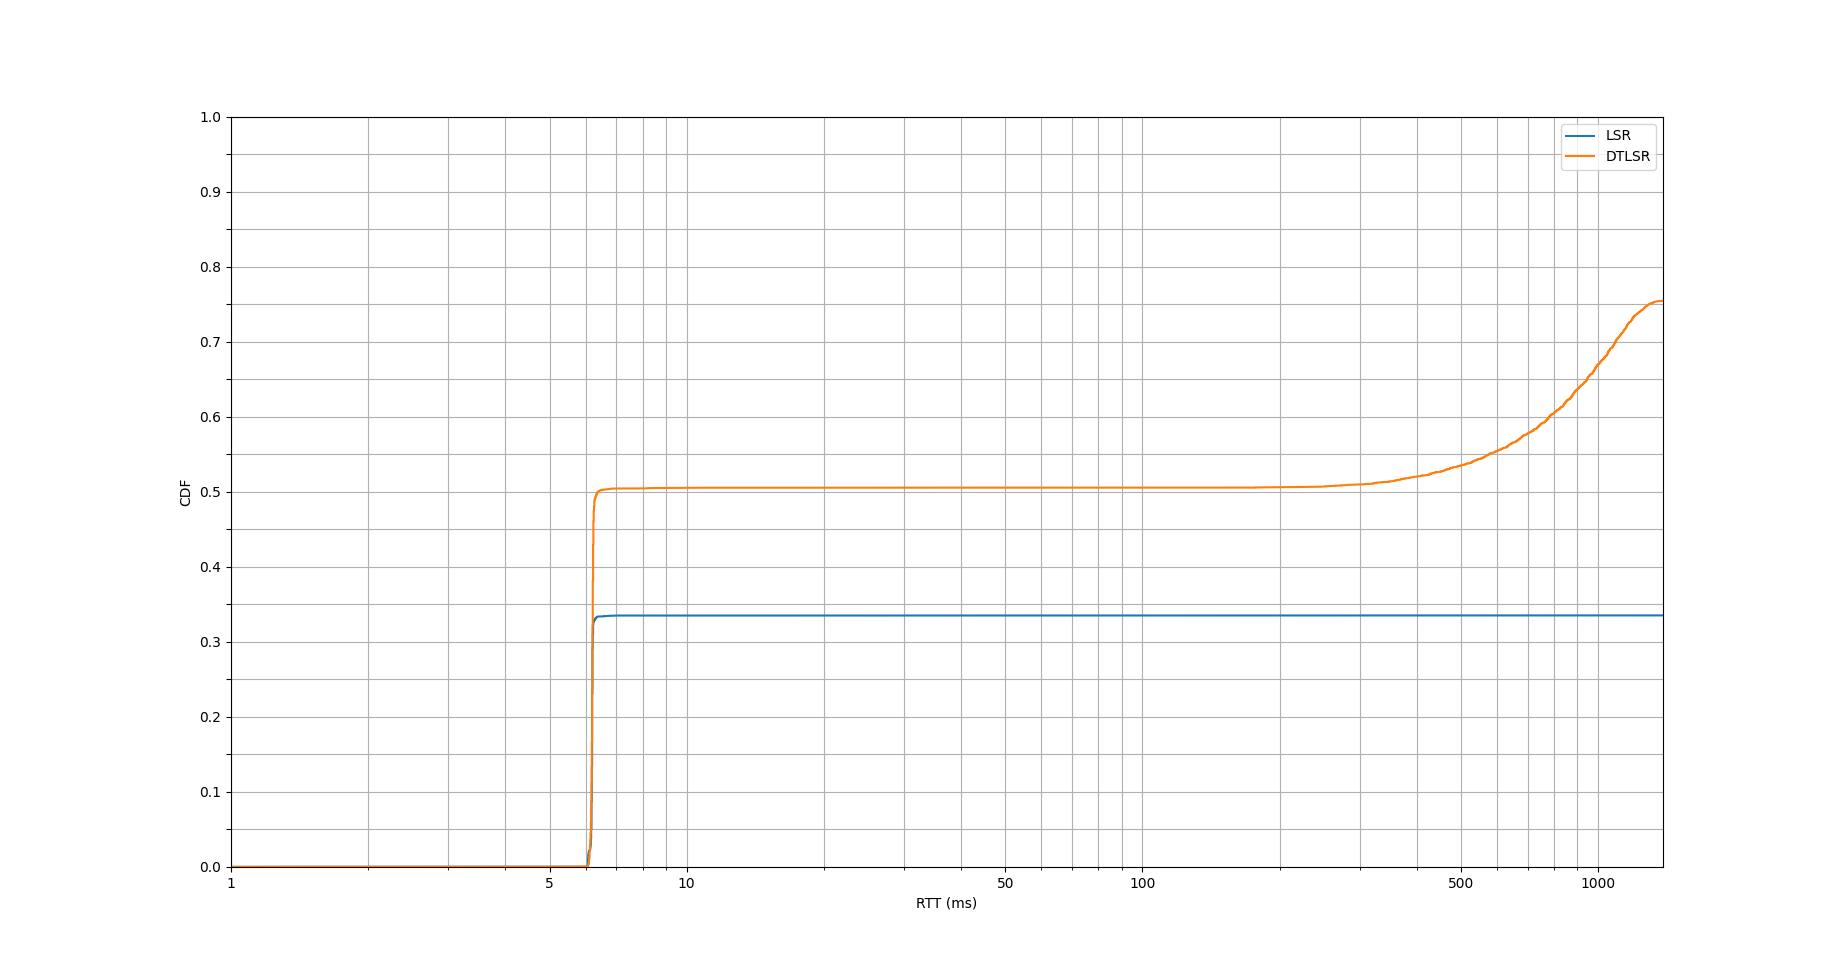
\includegraphics[width=190mm]{fig_partition_flap1} \\
  (a) Flapping with period $T=\SI{2}{\s}$ (\SI{1}{\s} up, \SI{1}{\s} down). \\ [6pt]
  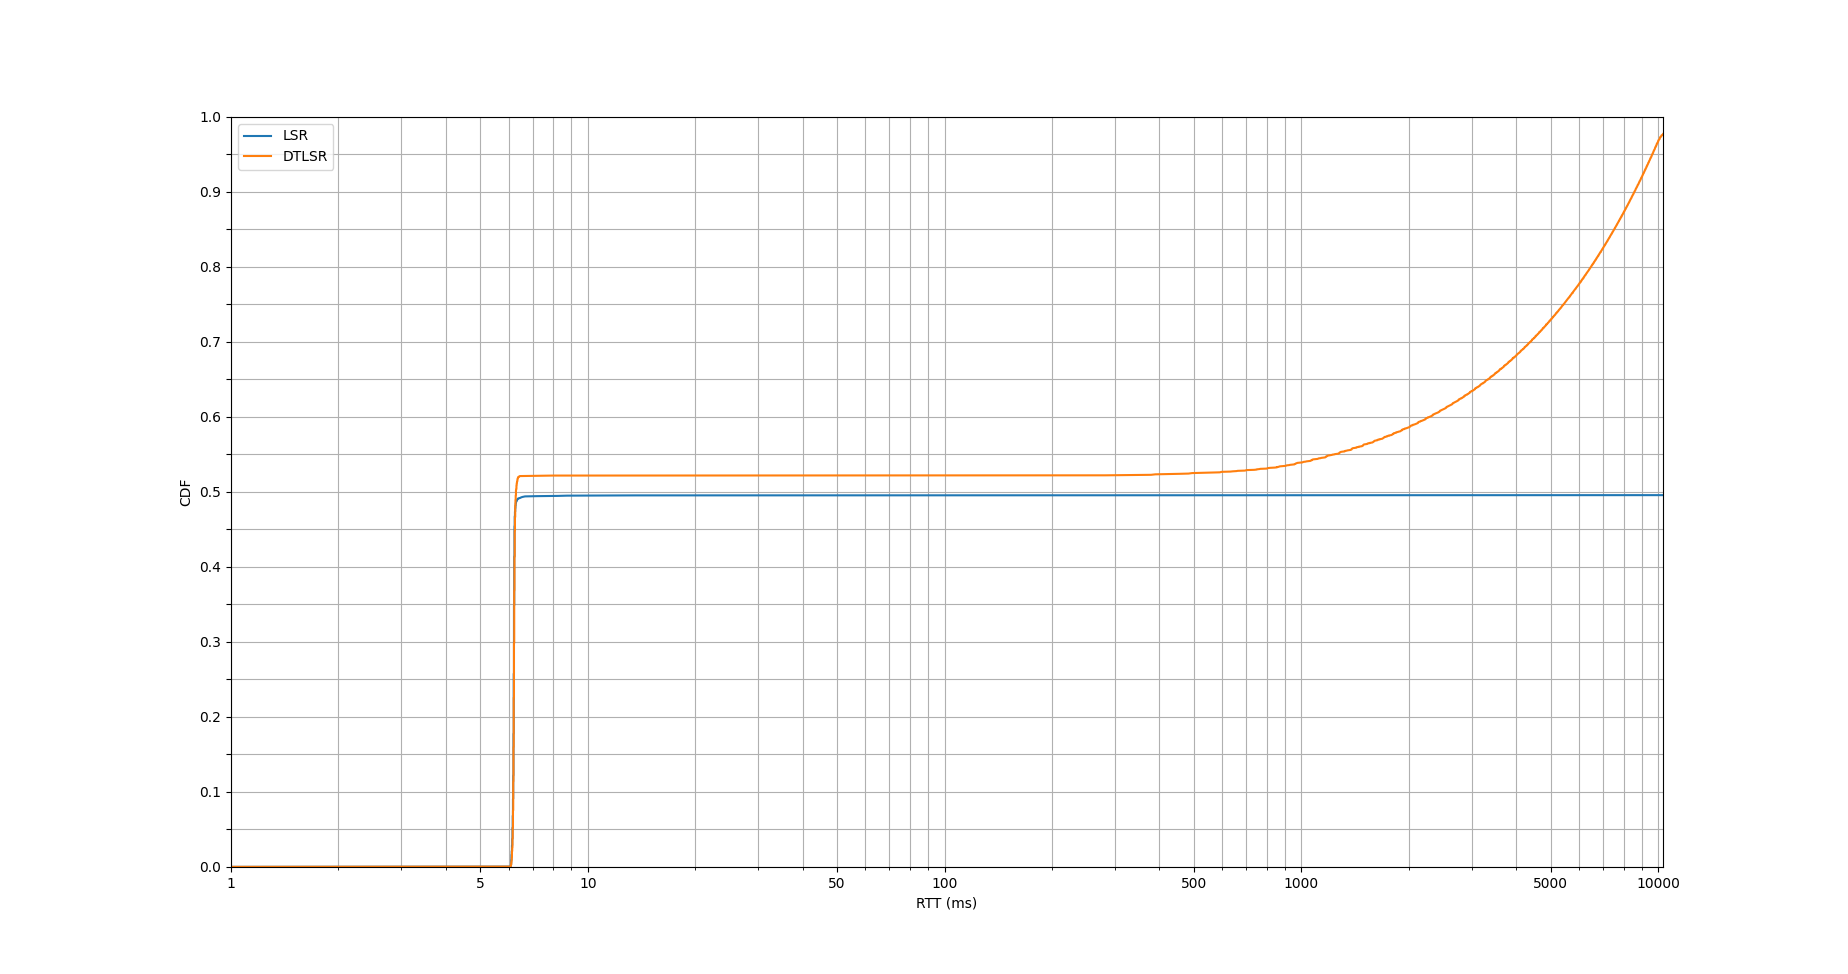
\includegraphics[width=190mm]{fig_partition_flap10} \\
  (b) Flapping with period $T=\SI{20}{\s}$ (\SI{10}{\s} up, \SI{10}{\s} down). \\[6pt]
\end{tabular}
\caption{Cumulative distributions of end-to-end delay between \texttt{n5} and \texttt{n6} under different routing algorithms, while flapping link \texttt{n1-n2}.}
\end{figure}

\pagebreak


Our second topology is a `box'-shaped one, where we have a low-delay main route and a higher delay backup route when the main one goes down. In this example \texttt{n1-n4} is the main link that we flap, and \texttt{n1-n2-n3-n4} is our higher-delay backup route. Every link has \SI{1}{\ms} of delay.

\begin{minipage}{1\textwidth} \centering
	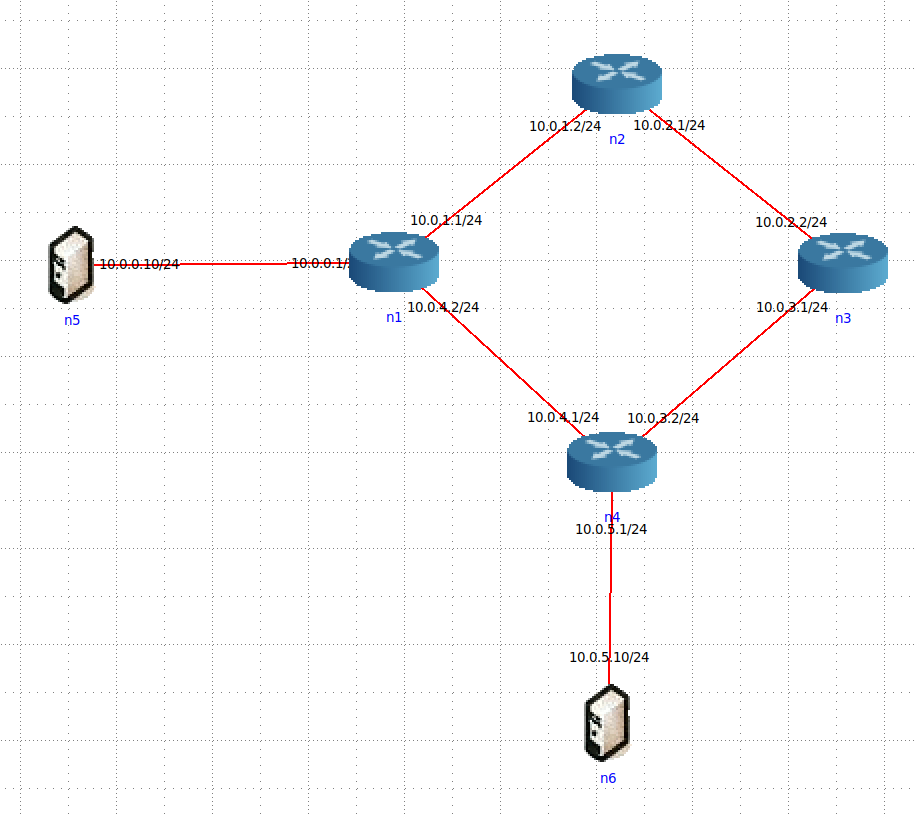
\includegraphics[width=0.7\textwidth]{box}
	\captionof{figure}{`Box' network topology.}
\end{minipage}

\begin{figure}
\begin{tabular}{c}
  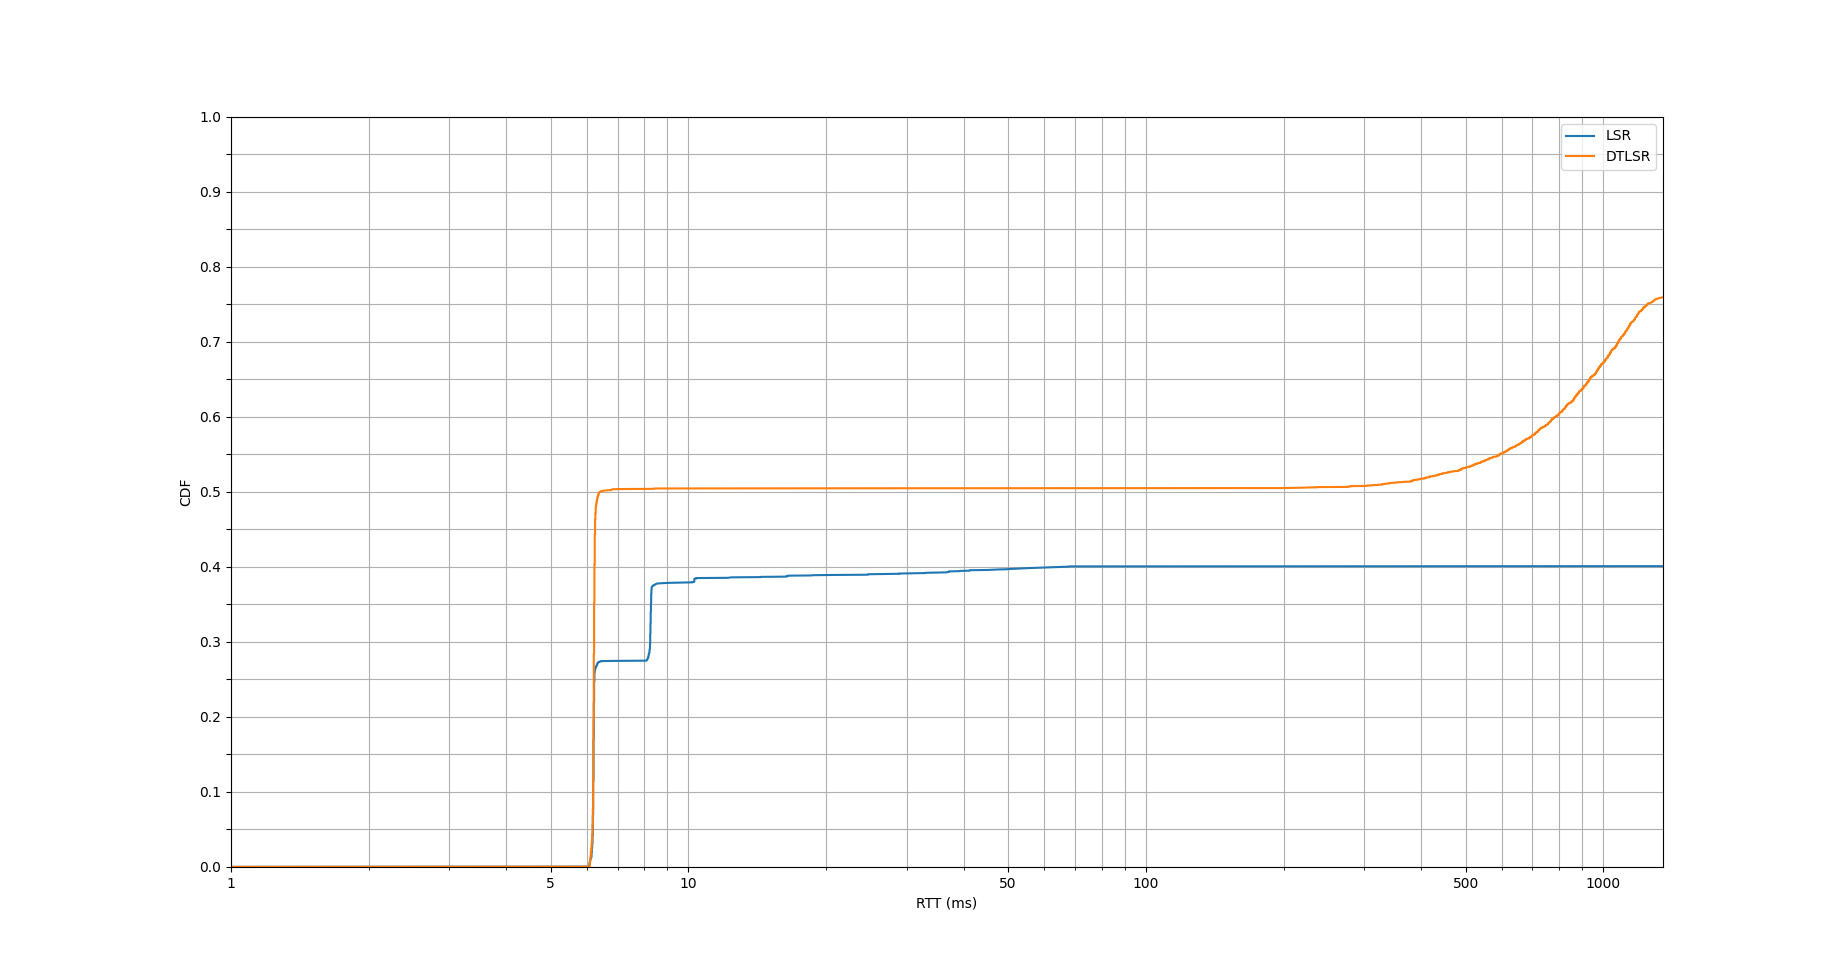
\includegraphics[width=190mm]{fig_box_flap1} \\
  (a) Flapping with period $T=\SI{2}{\s}$ (\SI{1}{\s} up, \SI{1}{\s} down). \\ [6pt]
  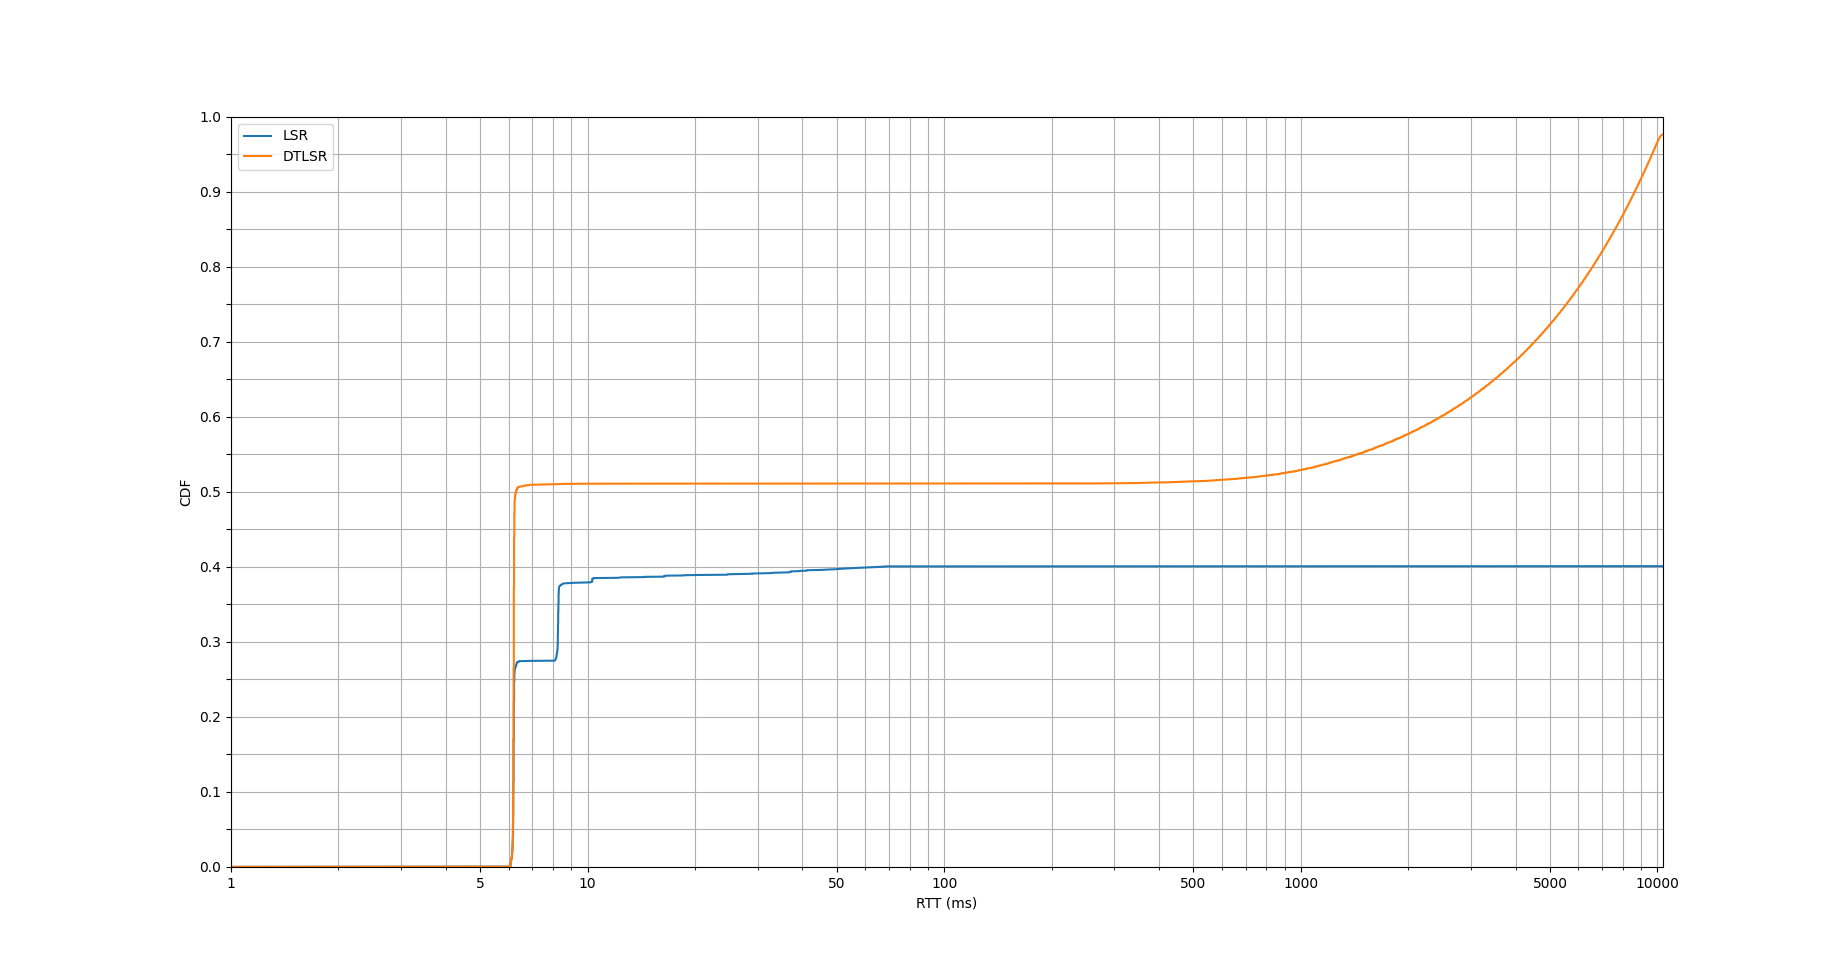
\includegraphics[width=190mm]{fig_box_flap10} \\
  (b) Flapping with period $T=\SI{20}{\s}$ (\SI{10}{\s} up, \SI{10}{\s} down). \\[6pt]
\end{tabular}
\caption{Cumulative distributions of end-to-end delay between \texttt{n5} and \texttt{n6} under different routing algorithms, while flapping link \texttt{n1-n4}.}
\end{figure}

\pagebreak

Our third topology is the same as the second, but we give the backup link a much higher delay than before. Every link has \SI{1}{\ms} of delay except for \texttt{n2-n3}, which has been set to have \SI{20}{\ms} of delay.

\section{Conclusions}

\section{Bibliography}

\section{Appendices}

\section{Index}

\section{Project Proposal}



\end{document}





























